\documentclass[../../../../main.tex]{subfiles}
\begin{document}

\begin{flushright}
\footnotesize\textit{【自動文字起こし・要確認】}
\end{flushright}

\begin{center}
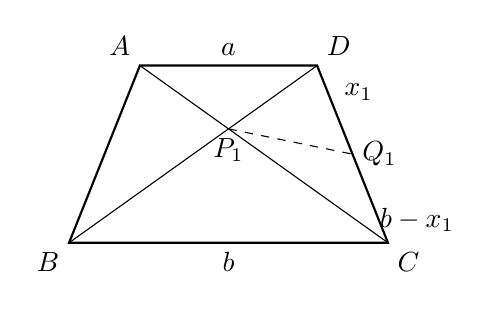
\begin{tikzpicture}[scale=0.9, >=stealth]
  % Top trapezoid diagram
  \coordinate (A) at (1,2.5);
  \coordinate (D) at (3.5,2.5);
  \coordinate (B) at (0,0);
  \coordinate (C) at (4.5,0);
  
  \draw[thick] (A) -- (D) -- (C) -- (B) -- cycle;
  \draw (A) -- (C);
  \draw (B) -- (D);
  
  % Intersection P1
  \coordinate (P1) at (intersection of A--C and B--D);
  \draw[dashed] (P1) -- (4.0, 1.25) coordinate (Q1);

  \node[above left] at (A) {$A$};
  \node[above right] at (D) {$D$};
  \node[below left] at (B) {$B$};
  \node[below right] at (C) {$C$};
  \node[below] at (P1) {$P_1$};
  \node[right] at (Q1) {$Q_1$};

  \node[above] at (2.25,2.5) {$a$};
  \node[below] at (2.25,0) {$b$};
  \node[above right] at (3.75, 1.875) {$x_1$};
  \node[below right] at (4.25, 0.625) {$b-x_1$};
\end{tikzpicture}

\vspace{0.5cm}

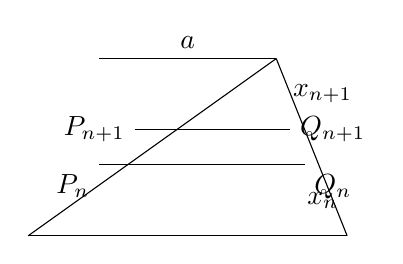
\begin{tikzpicture}[scale=0.9, >=stealth]
  % General step diagram
  \coordinate (A) at (1,2.5);
  \coordinate (D) at (3.5,2.5);
  \coordinate (B) at (0,0);
  \coordinate (C) at (4.5,0);

  \draw (A) -- (D);
  \draw (B) -- (C);
  \draw (B) -- (D);
  \draw (C) -- (D);

  \draw (1.5, 1.5) node[left] {$P_{n+1}$} -- (3.7, 1.5) node[right] {$Q_{n+1}$};
  \draw (1.0, 1.0) node[below left] {$P_n$} -- (3.9, 1.0) node[below right] {$Q_n$};

  \node[above] at (2.25,2.5) {$a$};
  \node[right] at (3.6, 2.0) {$x_{n+1}$};
  \node[right] at (3.8, 0.5) {$x_n$};
\end{tikzpicture}
\end{center}

\noindent
[\textbf{解}] (1) $B=P_0, C=Q_0$ とする。$\triangle P_n Q_n D$, $\triangle AD Q_n$ に注目し、相似から
\[
x_{n+1} : x_n - x_{n+1} = a - x_{n+1} : x_{n+1}
\]
\[
\therefore x_{n+1} = \frac{a x_n}{a + x_n} \tag{1}
\]
$x_n \neq 0$ だから、$y_n = \frac{1}{x_n}$ として、(1)の両辺逆数をとって、
\[
y_{n+1} = y_n + \frac{1}{a}
\]
$y_0 = \frac{1}{x_0} = \frac{1}{b}$ だから、くり返し用いて、
\[
y_n = \frac{n}{a} + \frac{1}{b}
\]
\[
\therefore x_n = \frac{1}{\frac{n}{a} + \frac{1}{b}} = \frac{ab}{a + bn}
\]

\noindent
(2) 辺 $P_{n+1} Q_{n+1}$ を底辺とみたときの $\triangle D P_{n+1} Q_n$ の高さ $h_n$ は
\[
h_n = \frac{H}{b} x_n \quad (n \ge 1)
\]
だから
\begin{align*}
F_n &= \frac{1}{2} h_n x_{n+1} = \frac{H}{2b} \cdot \frac{ab}{a+bn} \cdot \frac{ab}{a+b(n+1)} \\
&= \left( \frac{1}{a+bn} - \frac{1}{a+b(n+1)} \right) \frac{a^2 H}{2}
\end{align*}
となり、
\[
\sum_{k=1}^n F_k = \frac{a^2 H}{2} \left( \frac{1}{a+b} - \frac{1}{a+b(n+1)} \right) \xrightarrow{n \to \infty} \frac{H a^2}{2(a+b)}
\]

\newpage

\end{document}
